\documentclass[twoside,twocolumn,10pt]{article}
\usepackage{amssymb}
\usepackage{amsmath}
\usepackage{tikz}

\begin{document}

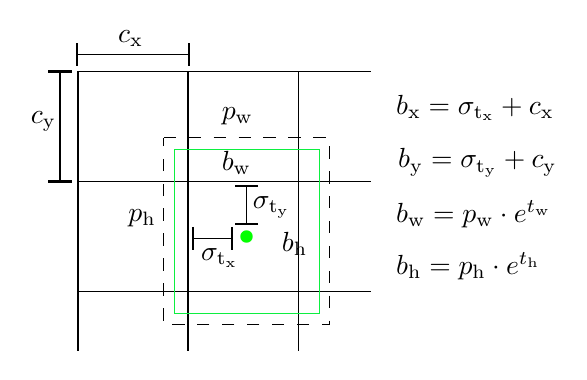
\begin{tikzpicture}[x=0.75pt,y=0.75pt,yscale=-1,xscale=1]

\draw  [draw opacity=0] (100,2905.81) -- (241.33,2905.81) -- (241.33,3040.48) -- (100,3040.48) -- cycle ; \draw   (100,2905.81) -- (100,3040.48)(153,2905.81) -- (153,3040.48)(206,2905.81) -- (206,3040.48) ; \draw   (100,2905.81) -- (241.33,2905.81)(100,2958.81) -- (241.33,2958.81)(100,3011.81) -- (241.33,3011.81) ; \draw    ;
\draw  [color={rgb, 255:red, 12; green, 239; blue, 64 }  ,draw opacity=1 ] (146.33,2943.31) -- (216.33,2943.31) -- (216.33,3022.31) -- (146.33,3022.31) -- cycle ;
\draw    (99.33,2897.81) -- (153.33,2897.81) ;
\draw [shift={(153.33,2897.81)}, rotate = 180] [color={rgb, 255:red, 0; green, 0; blue, 0 }  ][line width=0.75]    (0,5.59) -- (0,-5.59)   ;
\draw [shift={(99.33,2897.81)}, rotate = 180] [color={rgb, 255:red, 0; green, 0; blue, 0 }  ][line width=0.75]    (0,5.59) -- (0,-5.59)   ;
\draw    (91.33,2905.81) -- (91.33,2958.81) ;
\draw [shift={(91.33,2958.81)}, rotate = 270] [color={rgb, 255:red, 0; green, 0; blue, 0 }  ][line width=0.75]    (0,5.59) -- (0,-5.59)   ;
\draw [shift={(91.33,2905.81)}, rotate = 270] [color={rgb, 255:red, 0; green, 0; blue, 0 }  ][line width=0.75]    (0,5.59) -- (0,-5.59)   ;
\draw  [dash pattern={on 4.5pt off 4.5pt}] (141.33,2937.81) -- (221.33,2937.81) -- (221.33,3027.81) -- (141.33,3027.81) -- cycle ;
\draw  [draw opacity=0][fill={rgb, 255:red, 4; green, 255; blue, 0 }  ,fill opacity=1 ] (178.17,2985.31) .. controls (178.17,2983.66) and (179.51,2982.31) .. (181.17,2982.31) .. controls (182.82,2982.31) and (184.17,2983.66) .. (184.17,2985.31) .. controls (184.17,2986.97) and (182.82,2988.31) .. (181.17,2988.31) .. controls (179.51,2988.31) and (178.17,2986.97) .. (178.17,2985.31) -- cycle ;
\draw    (181.17,2960.81) -- (181.17,2979.31) ;
\draw [shift={(181.17,2979.31)}, rotate = 270] [color={rgb, 255:red, 0; green, 0; blue, 0 }  ][line width=0.75]    (0,5.59) -- (0,-5.59)   ;
\draw [shift={(181.17,2960.81)}, rotate = 270] [color={rgb, 255:red, 0; green, 0; blue, 0 }  ][line width=0.75]    (0,5.59) -- (0,-5.59)   ;
\draw    (155.33,2986.31) -- (174.17,2986.31) ;
\draw [shift={(174.17,2986.31)}, rotate = 180] [color={rgb, 255:red, 0; green, 0; blue, 0 }  ][line width=0.75]    (0,5.59) -- (0,-5.59)   ;
\draw [shift={(155.33,2986.31)}, rotate = 180] [color={rgb, 255:red, 0; green, 0; blue, 0 }  ][line width=0.75]    (0,5.59) -- (0,-5.59)   ;

% Text Node
\draw (118,2885) node [anchor=north west][inner sep=0.75pt]   [align=left] {$c_\mathrm{x}$};
% Text Node
\draw (76,2924) node [anchor=north west][inner sep=0.75pt]   [align=left] {$c_\mathrm{y}$};
% Text Node
\draw (183,2965) node [anchor=north west][inner sep=0.75pt]   [align=left] {$\sigma_\mathrm{t_\mathrm{y}}$};
% Text Node
\draw (158,2990) node [anchor=north west][inner sep=0.75pt]   [align=left] {$\sigma_\mathrm{t_\mathrm{x}}$};
% Text Node
\draw (168,2922) node [anchor=north west][inner sep=0.75pt]   [align=left] {$p_\mathrm{w}$};
% Text Node
\draw (123,2971) node [anchor=north west][inner sep=0.75pt]   [align=left] {$p_\mathrm{h}$};
% Text Node
\draw (168,2943) node [anchor=north west][inner sep=0.75pt]   [align=left] {$b_\mathrm{w}$};
% Text Node
\draw (197,2982) node [anchor=north west][inner sep=0.75pt]   [align=left] {$b_\mathrm{h}$};
% Text Node
\draw (252,2915.81) node [anchor=north west][inner sep=0.75pt]   [align=left] {$b_\mathrm{x} = \sigma_\mathrm{t_\mathrm{x}} + c_\mathrm{x} $};
% Text Node
\draw (253,2941.81) node [anchor=north west][inner sep=0.75pt]   [align=left] {$b_\mathrm{y} = \sigma_\mathrm{t_\mathrm{y}} + c_\mathrm{y} $};
% Text Node
\draw (252,2966.81) node [anchor=north west][inner sep=0.75pt]   [align=left] {$b_\mathrm{w} = p_\mathrm{w} \cdot e^{t_\mathrm{w}} $};
% Text Node
\draw (252,2991.81) node [anchor=north west][inner sep=0.75pt]   [align=left] {$b_\mathrm{h} = p_\mathrm{h} \cdot e^{t_\mathrm{h}} $};


\end{tikzpicture}

\end{document}